\subsection{Time Limit $(tl)$}
\label{sec:results_timelimit}
%
%\subsection{Accuracy evaluation}
%
%
In these experiments we evaluated the quality of the recommended visualizations produced by our proposed techniques 
 across different aggregate functions, namely: \texttt{count, sum, avg, min, max}. 
%
The dataset used is the Flights database with 10 dimension attributes and 10 measures attributes. 
%
We run these experiments to assess the quality of the recommended views over each aggregate function separately with a view space size $SP = 5 \times 10 \times 10 = 500$ possible views.
%
 A utility of a view is measured using the Earth Movers Distance (EMD).
%All Experiments were executed  5 times and obtained the averaged results, we concerned with evaluating the 

We report the accuracy, distance error and efficiency of views produced by our proposed algorithms by varying the time limits $tl$, number of views $R$ and $K$.
%
In these experiments, we use the following query:
%
\begin{center}
\texttt{$Q:$ SELECT * FROM Flights WHERE dimmonth IN ('APR','MAY','JUN'); }
\end{center}
%
%
The query $Q$  represents the  second quarter of the database, so that we can compare with the entire database to find different $K$ views while varying the time limit $tl$. 
%
In addition we evaluated the quality of the Top-$K$ views produced by each algorithm with those produced by SeeDB baseline, i.e., without any time limits or optimizations used. 
%and the average SeeDB baseline execution time is 23200ms.
% 
We implemented $SeeDB Timelimit$ algorithm which processes the entire data and views in a specified execution time limit, then recommends top views that are processed in that time limit.
%
This strategy represents a lower bound on accuracy and an upper bound on distance error.
%\mas{for all plots - use shades of grey, use one axis, use one metric per plot, and use straight lines not curves!}

In Figures \ref{fig:tlfig1} and \ref{fig:tlfig11}, the accuracy and distance error of the results produced by
algorithms $Sela$ , $Diff DVal$, $DimHisto$, and $SeeDB Timelimit$ to find a Top-100 $(K=100)$ views are compared with SeeDB baseline on different execution time limit $tl$. 
%
These algorithms output an ordered set of dimension attributes based on their priorities and submit the ordered set to the execution engine.
%
Then it processes all views generated according to the ordered set that produced by algorithms.
%
%\mas{and how did these algorithms become aware of the time limit?}
As shown, $SeeDB Timelimit$ shows high distance error and very low accuracy as well while the algorithms $Sela$ and $Diff DVal$ score higher accuracy than $DimHisto$. 
%
Although the proposed algorithms show a growing accuracy while extending the time limit, they achieved \%100 accuracy for $tl > 18000$ ms.
%
For a big database as the one used here (i.e., 500 different views), 18 seconds is considered reasonable.
%
%
%

The algorithms boosted the performance by more than \%30 and preserved the quality of views. 
%
On the other side, Figure \ref{fig:tlfig2} describes the execution costs referred to as the overhead time of the proposed algorithms on the same experiment. 
%
$DimHisto$ algorithm execution time is about 1200ms while the algorithms $Sela$ and $N-N'$ have almost the similar execution time, about 825ms. 
%\mas{is that overhead time or total time?!} 
This shows that $Sela$ and $Diff DVal$ algorithms are faster by \%66 than $DimHisto$. 
%
As discussed previously, the additional histograms distance computations are the cause of the extra overhead in algorithm $DimHisto$. 
%
\begin{figure}[t]
  \begin{subfigure}[b]{0.32\textwidth}
    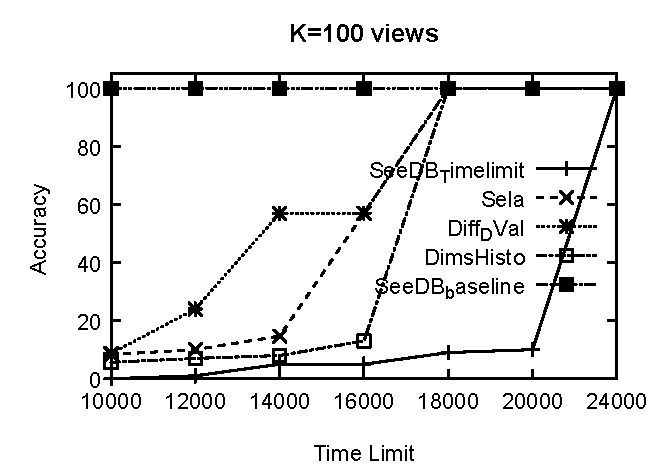
\includegraphics[width=\textwidth]{tl1.pdf}
    \caption{Accuracy}
        \label{fig:tlfig1}%
  \end{subfigure}
	\begin{subfigure}[b]{0.32\textwidth}
    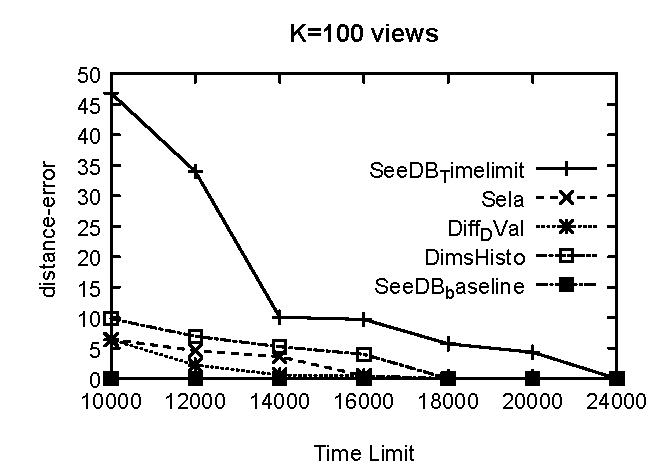
\includegraphics[width=\textwidth]{tl11.pdf}
    \caption{Distance error}
        \label{fig:tlfig11}%
  \end{subfigure}
  %
  \begin{subfigure}[b]{0.32\textwidth}
    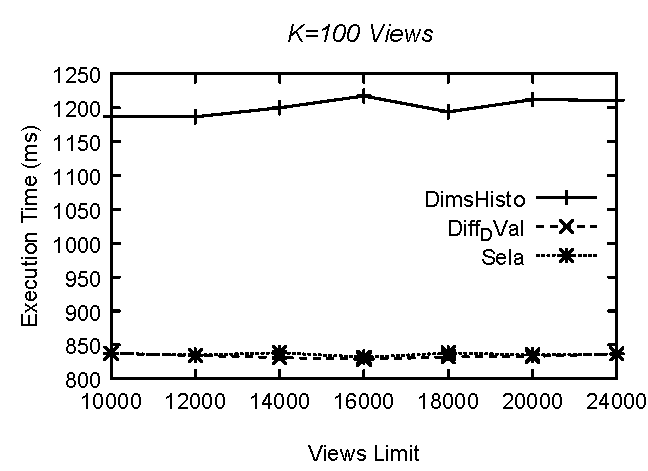
\includegraphics[width=\textwidth]{tl2.pdf}
     \caption{Average overhead}
        \label{fig:tlfig2}
  \end{subfigure}
  \caption{Performance of $Sela$ , $Diff DVal$, $DimHisto$, and $SeeDB Timelimit$ on different time limits while $K=100$}
\end{figure}

 %\begin{figure}[h]
%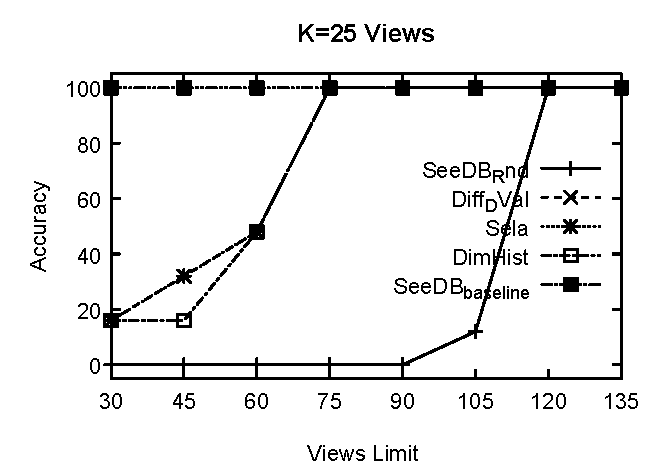
\includegraphics[width=\textwidth]{21.pdf}
%\caption{Accuracy compared with  the view space size for the Algorithms $Sela$ , $N-N'$, $DimHisto$, and $SeeDB_Rnd$}
%\label{fig:fig1}%
%\end{figure}



%\begin{figure}[h]
%\includegraphics[width=\textwidth]{{22.pdf}}
%\caption{Error Distance according to the view space size for the Algorithms $Sela$ , $N-N'$, $DimHisto$, and $SeeDB_Rnd$}
%\label{fig:figa2}%
%\end{figure}

  
%  \begin{figure}[h]
%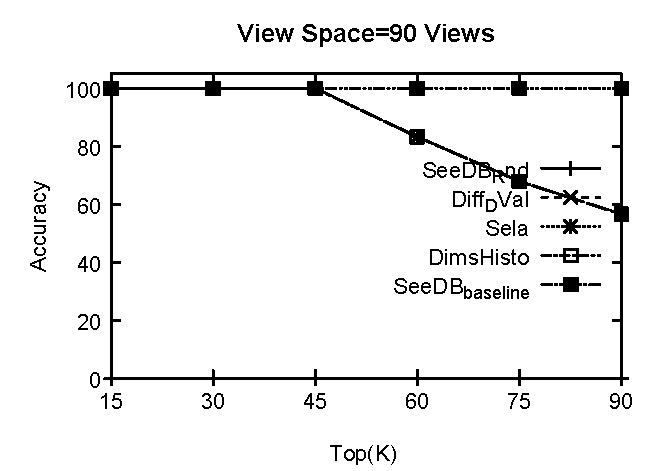
\includegraphics[width=\textwidth]{11.pdf}
%\caption{Accuracy compared with  top(K) views for the Algorithms $Sela$ , $N-N'$, $DimHisto$, and $SeeDB_Rnd$}
%\label{fig:fig3}%
%\end{figure}

\begin{figure}[t]
  \begin{subfigure}[b]{0.32\textwidth}
    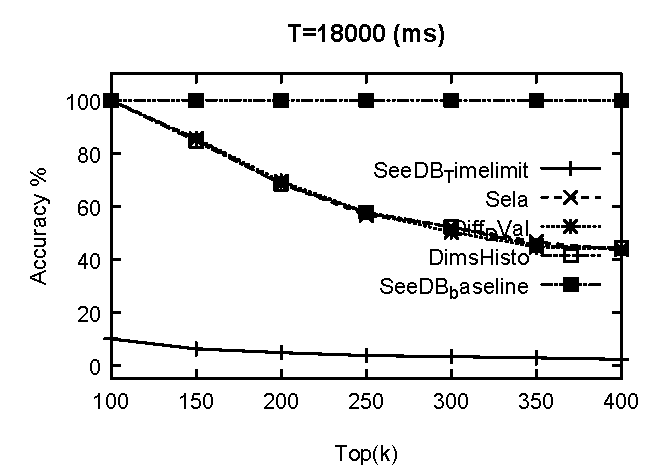
\includegraphics[width=\textwidth]{tl3.pdf}
    \caption{Accuracy }
       \label{fig:tlfig3}
  \end{subfigure}
	\begin{subfigure}[b]{0.32\textwidth}
    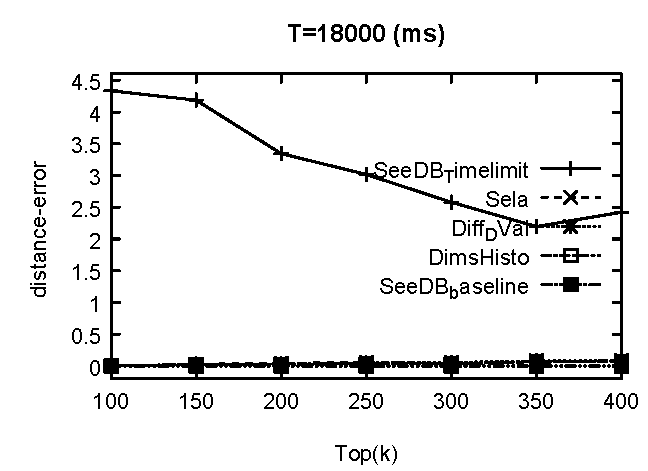
\includegraphics[width=\textwidth]{tl31.pdf}
    \caption{Distance error}
       \label{fig:tlfig31}
  \end{subfigure}
  %
  \begin{subfigure}[b]{0.32\textwidth}
    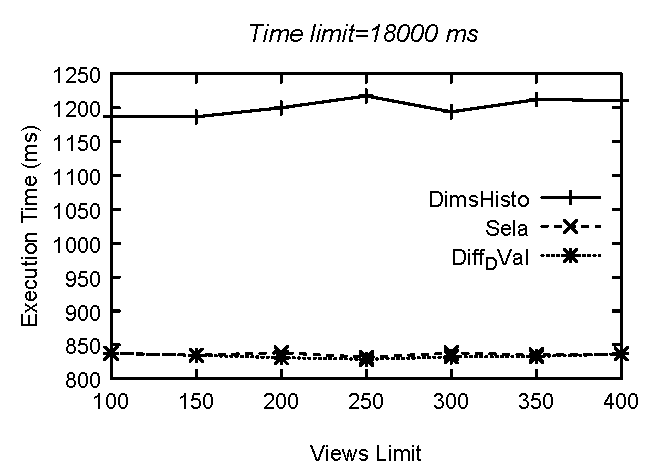
\includegraphics[width=\textwidth]{tl4.pdf}
     \caption{Average overhead}
       \label{fig:tlfig4}%
  \end{subfigure}
  \caption{Performance of$Sela$ , $Diff DVal$, $DimHisto$, and $SeeDB Timelimit$ on varying $K$ and $tl=18$s}
\end{figure}
%
To show the effects of varying $K$ with time limits, Figures \ref{fig:tlfig3} and \ref{fig:tlfig31} show the accuracy of the 
algorithms $Sela$ , $N-N'$, $DimHisto$, and $SeeDB Timelimit$ in a certain time limit $tl=18000$ms.
%
As shown, all algorithms score \%100 accuracy in the first top 100 views. 
%
However, the accuracy declines with increasing $K$ while $tl$ is fixed, but the proposed algorithms score very small distance error for large values of $K$ while $SeeDB Timelimit$ shows very low accuracy and huge distance error. 
%
As illustrated in Figure \ref{fig:tlfig2}, the overhead costs of the proposed algorithms remain stable on different time limits. 
 %
In short, the proposed algorithms improve the quality of the results, thanks to the evaluation metrics that are used along different $K$, $R$ and times limits $tl$ values. 
%
Moreover, the algorithms overhead is comparatively small with the total execution time of baseline SeeDB.
%\begin{figure}[t]
%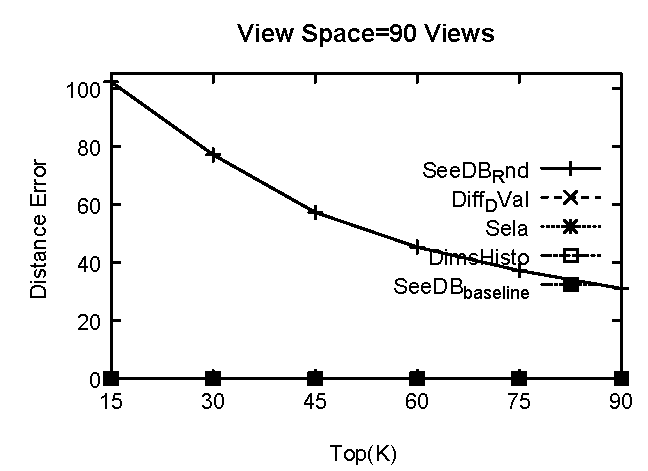
\includegraphics[width=\textwidth]{12.pdf}
%\caption{Error Distance compared with  the view space size for the Algorithms $Sela$ , $N-N'$, $DimHisto$, and $SeeDB_Rnd$}
%\label{fig:fig4}%
%\end{figure}
